
\chapter{Formal specification of the gameplay}
\label{chap:formal}

\section{Grid universe}

The universe is made of a $m$ (horizontally) by $n$ (vertically) array of cases.
The cases are delimited by a grid.
We represent those with planar graphs:
\begin{itemize}
    \item The array of cases: $G_A = (V_A, E_A)$, with
        \begin{align*}
            V_A &= \left\{v_{a,ij} : 0 \le i < m, 0 \le j < n\right\} \\
            E_A &= \left\{\{v_{a,i_1j_1}, v_{a,i_2,j_2}\} :
            |i_1-i_2| + |j_1-j_2| = 1 \right\}
        \end{align*}
    \item The grid: $G_G = (V_G, E_G)$, with
        \[V_G = \left\{v_{g,ij} : 0 \le i \le m, 0 \le j \le n\right\} \]
        \[
            \begin{split}
                E_G = \{
                    \{v_{g,i_1j_1}, v_{g,i_2,j_2}\} :
                    & |i_1-i_2| + |j_1-j_2| = 1; \\
                    & 0 < i_1 < m; 0 < j_1 < n; \\
                    & 0 \le i_2 \le m, 0 \le j_2 \le n
                \}
            \end{split}
        \]
\end{itemize}
The graphs are depicted in figure~\ref{fig:graphs1}.
\begin{figure}
    \begin{center}
        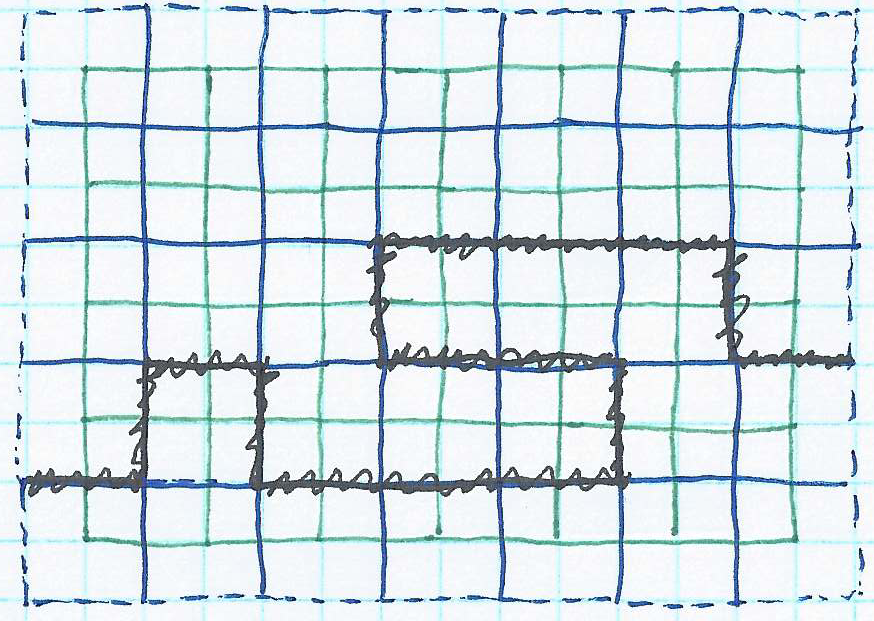
\includegraphics[width=0.3\textwidth]{img/graphs_universe_draft.png}
    \end{center}
    \caption{Representation of the graphs: $G_A$ is in green, $G_G$ in blue
        (the dashed blue lines are not edges of the graph) and the global border
        in black.
    }
    \label{fig:graphs1}
\end{figure}
On this representation, all the edges of $G_G$ intersect
edges of $G_A$, which gives a correspondance bijection $c:E_G \rightarrow E_A$,
formally defined as follows
\begin{align*}
    c(\{v_{g,i,j}, v_{g,i+1,j}\}) &= \{v_{a,i,j-1}, v_{a,i,j}\} \\
    c(\{v_{g,i,j}, v_{g,i,j+1}\}) &= \{v_{a,i-1,j}, v_{a,i,j}\}.
\end{align*}

A border $B$ is a path in $G_G$, which starts at $v_{g,0j}$ and ends at
$v_{g,m+1,j'}$.

Due to the structure of both graphs, the edges of the border corresponds
(by $c$) to a set for edges which form a cut of $G_A$. This cut defines
two subgraphs: the free space $F$ (containing cases $v_{a,i,n-1}$) and
the structure $S$ (containing cases $v_{a,i0}$).

The following properties hold for any border:
\begin{itemize}
    \item the free space contains the upper row $v_{a,i,n-1}$;
    \item the structure contains the lower row of cases $v_{a,i0}$;
    \item the structure is connex;
    \item the free space is connex.
\end{itemize}

$F$ and $S$ are complementary, there is thus an trivial bijection between
the set of free spaces and the set of structures.

A free space, structure pair  which satisfies the preceding properties
is said to be well-formed.

A well-formed free space, structure pair always corresponds to a border:
taking the edges in $G_G$ corresponding to the edges of $G_A$
linking the structure and the free space gives
a set of edges which constitue a border.
There is thus a bijection between borders and well-formed free spaces (and structures).

\section{Players}

There is a global well-formed structure which is the same for all the players.
For all cases $v_{a,i,j}$ in the global structure, the condition $j < n - N_p$
must hold, where $N_p$ is the number of players.

The structure is thus conceptually dense (not holes in it). But this
does not imply anything on the display: the inner cases of the structure
can be anything, this doesn't impact the gameplay.

Each player $p_k, 0\le k < N_p$ is an entity, that occupies a case $v_{a,p_k}$.
Cases occupied by players must be in the global free space (ie. outside the global
structure). Only one player may occupy a given place at a given time.

Each player must be hooked to a neighbour case, which must be either occupied by
the global structure, either by another player. In any set of players, there must
be at least one player hooked to a case occupied by the global structure.

The hook point is the edge linking the case occupied by the player and the case
it is hooked to (or the corresponding edge through the bijection $c$).

\section{Movements}

At any time, each player has its own free space, structure, border triple $(F_k, S_k, B_k)$.
The free space is the largest connex component that contains the cases of the upper row,
but no cases of the global structure, and no cases occupied by other players.
The definition of its structure and border follows from that.

From the border $B_k$, extracting the edges gives a sequence of hook points $(h_k)_i$.
The player is always hooked to a point in this sequence.
To each hook point corresponds a unique case that can be occupied by the player
(the converse is not true).

When a player moves right, its new hook point is determined in two steps:
\begin{enumerate}
    \item Finding new case: from the current hook point, $(h_k)_i$ is traversed
        (increasing $i$), until the traversed hook point corresponds to a case
        different of the current case of the player. If no such hook point is
        found before the end of the sequence, the move is impossible.
    \item Deciding the new hook point: if possible, the player hooks to the
        global structure. To do this, the list is traversed, from the hook
        point found at previous step. One switches to the next hook point if
        the next hook point corrsponds to the same case as the same hook point
        and if the current hook point is hooking on another player. Otherwise,
        the traversing stops.
\end{enumerate}

\section{Mask}

The mask is a set of cases which must include all the cases of the global
structure. The connex component of the mask containing the global structure
must also include at least $N_p$ cases of the global free space.

